\documentclass[1p]{elsarticle_modified}
%\bibliographystyle{elsarticle-num}

%\usepackage[colorlinks]{hyperref}
%\usepackage{abbrmath_seonhwa} %\Abb, \Ascr, \Acal ,\Abf, \Afrak
\usepackage{amsfonts}
\usepackage{amssymb}
\usepackage{amsmath}
\usepackage{amsthm}
\usepackage{scalefnt}
\usepackage{amsbsy}
\usepackage{kotex}
\usepackage{caption}
\usepackage{subfig}
\usepackage{color}
\usepackage{graphicx}
\usepackage{xcolor} %% white, black, red, green, blue, cyan, magenta, yellow
\usepackage{float}
\usepackage{setspace}
\usepackage{hyperref}

\usepackage{tikz}
\usetikzlibrary{arrows}

\usepackage{multirow}
\usepackage{array} % fixed length table
\usepackage{hhline}

%%%%%%%%%%%%%%%%%%%%%
\makeatletter
\renewcommand*\env@matrix[1][\arraystretch]{%
	\edef\arraystretch{#1}%
	\hskip -\arraycolsep
	\let\@ifnextchar\new@ifnextchar
	\array{*\c@MaxMatrixCols c}}
\makeatother %https://tex.stackexchange.com/questions/14071/how-can-i-increase-the-line-spacing-in-a-matrix
%%%%%%%%%%%%%%%

\usepackage[normalem]{ulem}

\newcommand{\msout}[1]{\ifmmode\text{\sout{\ensuremath{#1}}}\else\sout{#1}\fi}
%SOURCE: \msout is \stkout macro in https://tex.stackexchange.com/questions/20609/strikeout-in-math-mode

\newcommand{\cancel}[1]{
	\ifmmode
	{\color{red}\msout{#1}}
	\else
	{\color{red}\sout{#1}}
	\fi
}

\newcommand{\add}[1]{
	{\color{blue}\uwave{#1}}
}

\newcommand{\replace}[2]{
	\ifmmode
	{\color{red}\msout{#1}}{\color{blue}\uwave{#2}}
	\else
	{\color{red}\sout{#1}}{\color{blue}\uwave{#2}}
	\fi
}

\newcommand{\Sol}{\mathcal{S}} %segment
\newcommand{\D}{D} %diagram
\newcommand{\A}{\mathcal{A}} %arc


%%%%%%%%%%%%%%%%%%%%%%%%%%%%%5 test

\def\sl{\operatorname{\textup{SL}}(2,\Cbb)}
\def\psl{\operatorname{\textup{PSL}}(2,\Cbb)}
\def\quan{\mkern 1mu \triangleright \mkern 1mu}

\theoremstyle{definition}
\newtheorem{thm}{Theorem}[section]
\newtheorem{prop}[thm]{Proposition}
\newtheorem{lem}[thm]{Lemma}
\newtheorem{ques}[thm]{Question}
\newtheorem{cor}[thm]{Corollary}
\newtheorem{defn}[thm]{Definition}
\newtheorem{exam}[thm]{Example}
\newtheorem{rmk}[thm]{Remark}
\newtheorem{alg}[thm]{Algorithm}

\newcommand{\I}{\sqrt{-1}}
\begin{document}

%\begin{frontmatter}
%
%\title{Boundary parabolic representations of knots up to 8 crossings}
%
%%% Group authors per affiliation:
%\author{Yunhi Cho} 
%\address{Department of Mathematics, University of Seoul, Seoul, Korea}
%\ead{yhcho@uos.ac.kr}
%
%
%\author{Seonhwa Kim} %\fnref{s_kim}}
%\address{Center for Geometry and Physics, Institute for Basic Science, Pohang, 37673, Korea}
%\ead{ryeona17@ibs.re.kr}
%
%\author{Hyuk Kim}
%\address{Department of Mathematical Sciences, Seoul National University, Seoul 08826, Korea}
%\ead{hyukkim@snu.ac.kr}
%
%\author{Seokbeom Yoon}
%\address{Department of Mathematical Sciences, Seoul National University, Seoul, 08826,  Korea}
%\ead{sbyoon15@snu.ac.kr}
%
%\begin{abstract}
%We find all boundary parabolic representation of knots up to 8 crossings.
%
%\end{abstract}
%\begin{keyword}
%    \MSC[2010] 57M25 
%\end{keyword}
%
%\end{frontmatter}

%\linenumbers
%\tableofcontents
%
\newcommand\colored[1]{\textcolor{white}{\rule[-0.35ex]{0.8em}{1.4ex}}\kern-0.8em\color{red} #1}%
%\newcommand\colored[1]{\textcolor{white}{ #1}\kern-2.17ex	\textcolor{white}{ #1}\kern-1.81ex	\textcolor{white}{ #1}\kern-2.15ex\color{red}#1	}

{\Large $\underline{12n_{0558}~(K12n_{0558})}$}

\setlength{\tabcolsep}{10pt}
\renewcommand{\arraystretch}{1.6}
\vspace{1cm}\begin{tabular}{m{100pt}>{\centering\arraybackslash}m{274pt}}
\multirow{5}{120pt}{
	\centering
	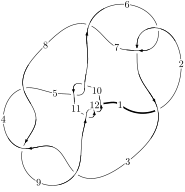
\includegraphics[width=112pt]{../../../GIT/diagram.site/Diagrams/png/2647_12n_0558.png}\\
\ \ \ A knot diagram\footnotemark}&
\allowdisplaybreaks
\textbf{Linearized knot diagam} \\
\cline{2-2}
 &
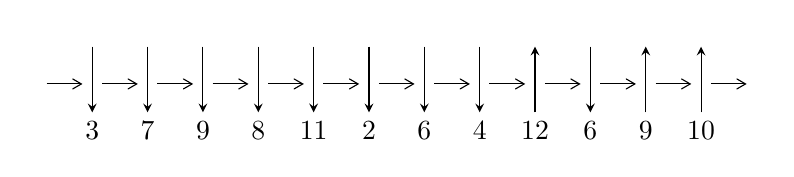
\begin{tikzpicture}[x=20pt, y=17pt]
	% nodes
	\node (C0) at (0, 0) {};
	\node (C1) at (1, 0) {};
	\node (C1U) at (1, +1) {};
	\node (C1D) at (1, -1) {3};

	\node (C2) at (2, 0) {};
	\node (C2U) at (2, +1) {};
	\node (C2D) at (2, -1) {7};

	\node (C3) at (3, 0) {};
	\node (C3U) at (3, +1) {};
	\node (C3D) at (3, -1) {9};

	\node (C4) at (4, 0) {};
	\node (C4U) at (4, +1) {};
	\node (C4D) at (4, -1) {8};

	\node (C5) at (5, 0) {};
	\node (C5U) at (5, +1) {};
	\node (C5D) at (5, -1) {11};

	\node (C6) at (6, 0) {};
	\node (C6U) at (6, +1) {};
	\node (C6D) at (6, -1) {2};

	\node (C7) at (7, 0) {};
	\node (C7U) at (7, +1) {};
	\node (C7D) at (7, -1) {6};

	\node (C8) at (8, 0) {};
	\node (C8U) at (8, +1) {};
	\node (C8D) at (8, -1) {4};

	\node (C9) at (9, 0) {};
	\node (C9U) at (9, +1) {};
	\node (C9D) at (9, -1) {12};

	\node (C10) at (10, 0) {};
	\node (C10U) at (10, +1) {};
	\node (C10D) at (10, -1) {6};

	\node (C11) at (11, 0) {};
	\node (C11U) at (11, +1) {};
	\node (C11D) at (11, -1) {9};

	\node (C12) at (12, 0) {};
	\node (C12U) at (12, +1) {};
	\node (C12D) at (12, -1) {10};
	\node (C13) at (13, 0) {};

	% arrows
	\draw[->,>={angle 60}]
	(C0) edge (C1) (C1) edge (C2) (C2) edge (C3) (C3) edge (C4) (C4) edge (C5) (C5) edge (C6) (C6) edge (C7) (C7) edge (C8) (C8) edge (C9) (C9) edge (C10) (C10) edge (C11) (C11) edge (C12) (C12) edge (C13) ;	\draw[->,>=stealth]
	(C1U) edge (C1D) (C2U) edge (C2D) (C3U) edge (C3D) (C4U) edge (C4D) (C5U) edge (C5D) (C6U) edge (C6D) (C7U) edge (C7D) (C8U) edge (C8D) (C9D) edge (C9U) (C10U) edge (C10D) (C11D) edge (C11U) (C12D) edge (C12U) ;
	\end{tikzpicture} \\
\hhline{~~} \\& 
\textbf{Solving Sequence} \\ \cline{2-2} 
 &
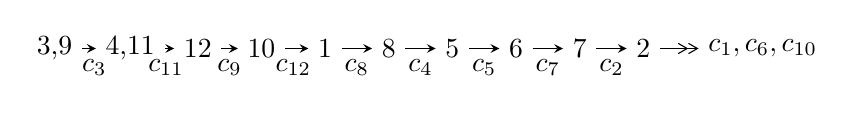
\begin{tikzpicture}[x=23pt, y=7pt]
	% node
	\node (A0) at (-1/8, 0) {3,9};
	\node (A1) at (17/16, 0) {4,11};
	\node (A2) at (17/8, 0) {12};
	\node (A3) at (25/8, 0) {10};
	\node (A4) at (33/8, 0) {1};
	\node (A5) at (41/8, 0) {8};
	\node (A6) at (49/8, 0) {5};
	\node (A7) at (57/8, 0) {6};
	\node (A8) at (65/8, 0) {7};
	\node (A9) at (73/8, 0) {2};
	\node (C1) at (1/2, -1) {$c_{3}$};
	\node (C2) at (13/8, -1) {$c_{11}$};
	\node (C3) at (21/8, -1) {$c_{9}$};
	\node (C4) at (29/8, -1) {$c_{12}$};
	\node (C5) at (37/8, -1) {$c_{8}$};
	\node (C6) at (45/8, -1) {$c_{4}$};
	\node (C7) at (53/8, -1) {$c_{5}$};
	\node (C8) at (61/8, -1) {$c_{7}$};
	\node (C9) at (69/8, -1) {$c_{2}$};
	\node (A10) at (11, 0) {$c_{1},c_{6},c_{10}$};

	% edge
	\draw[->,>=stealth]	
	(A0) edge (A1) (A1) edge (A2) (A2) edge (A3) (A3) edge (A4) (A4) edge (A5) (A5) edge (A6) (A6) edge (A7) (A7) edge (A8) (A8) edge (A9) ;
	\draw[->>,>={angle 60}]	
	(A9) edge (A10);
\end{tikzpicture} \\ 

\end{tabular} \\

\footnotetext{
The image of knot diagram is generated by the software ``\textbf{Draw programme}" developed by Andrew Bartholomew(\url{http://www.layer8.co.uk/maths/draw/index.htm\#Running-draw}), where we modified some parts for our purpose(\url{https://github.com/CATsTAILs/LinksPainter}).
}\phantom \\ \newline 
\centering \textbf{Ideals for irreducible components\footnotemark of $X_{\text{par}}$} 
 
\begin{align*}
I^u_{1}&=\langle 
6.38928\times10^{32} u^{29}-1.63982\times10^{33} u^{28}+\cdots+2.11658\times10^{34} b+1.61565\times10^{34},\\
\phantom{I^u_{1}}&\phantom{= \langle  }-5.75591\times10^{32} u^{29}+4.74067\times10^{32} u^{28}+\cdots+6.34974\times10^{34} a+7.64726\times10^{34},\\
\phantom{I^u_{1}}&\phantom{= \langle  }u^{30}-2 u^{29}+\cdots-36 u-36\rangle \\
I^u_{2}&=\langle 
u^4- u^3+3 u^2+b-3 u,\;- u^4+u^3-4 u^2+a+3 u-3,\;u^5- u^4+4 u^3-3 u^2+3 u-1\rangle \\
I^u_{3}&=\langle 
b a u+b^2+2 b a-2 b u+b+a-2 u,\;a^2- a u+1,\;u^2+1\rangle \\
\\
\end{align*}
\raggedright * 3 irreducible components of $\dim_{\mathbb{C}}=0$, with total 43 representations.\\
\footnotetext{All coefficients of polynomials are rational numbers. But the coefficients are sometimes approximated in decimal forms when there is not enough margin.}
\newpage
\renewcommand{\arraystretch}{1}
\centering \section*{I. $I^u_{1}= \langle 6.39\times10^{32} u^{29}-1.64\times10^{33} u^{28}+\cdots+2.12\times10^{34} b+1.62\times10^{34},\;-5.76\times10^{32} u^{29}+4.74\times10^{32} u^{28}+\cdots+6.35\times10^{34} a+7.65\times10^{34},\;u^{30}-2 u^{29}+\cdots-36 u-36 \rangle$}
\flushleft \textbf{(i) Arc colorings}\\
\begin{tabular}{m{7pt} m{180pt} m{7pt} m{180pt} }
\flushright $a_{3}=$&$\begin{pmatrix}1\\0\end{pmatrix}$ \\
\flushright $a_{9}=$&$\begin{pmatrix}0\\u\end{pmatrix}$ \\
\flushright $a_{4}=$&$\begin{pmatrix}1\\u^2\end{pmatrix}$ \\
\flushright $a_{11}=$&$\begin{pmatrix}0.00906479 u^{29}-0.00746591 u^{28}+\cdots-3.45875 u-1.20434\\-0.0301868 u^{29}+0.0774751 u^{28}+\cdots+0.497856 u-0.763331\end{pmatrix}$ \\
\flushright $a_{12}=$&$\begin{pmatrix}0.00906479 u^{29}-0.00746591 u^{28}+\cdots-3.45875 u-1.20434\\-0.0230609 u^{29}+0.0603049 u^{28}+\cdots-0.212369 u-1.14722\end{pmatrix}$ \\
\flushright $a_{10}=$&$\begin{pmatrix}-0.0180236 u^{29}+0.0235211 u^{28}+\cdots-1.46858 u+0.229478\\-0.0262408 u^{29}+0.0578653 u^{28}+\cdots+0.566767 u-0.217670\end{pmatrix}$ \\
\flushright $a_{1}=$&$\begin{pmatrix}-0.00197135 u^{29}-0.0109705 u^{28}+\cdots-0.133902 u+1.62976\\-0.0140099 u^{29}+0.0220006 u^{28}+\cdots+1.02890 u+0.106895\end{pmatrix}$ \\
\flushright $a_{8}=$&$\begin{pmatrix}u\\u^3+u\end{pmatrix}$ \\
\flushright $a_{5}=$&$\begin{pmatrix}u^2+1\\u^4+2 u^2\end{pmatrix}$ \\
\flushright $a_{6}=$&$\begin{pmatrix}0.0118634 u^{29}-0.0426200 u^{28}+\cdots-1.74552 u+0.488618\\0.00457667 u^{29}+0.00334632 u^{28}+\cdots-2.20933 u-1.11355\end{pmatrix}$ \\
\flushright $a_{7}=$&$\begin{pmatrix}-0.0141492 u^{29}+0.0501839 u^{28}+\cdots+1.57769 u-1.21616\\0.0122465 u^{29}-0.0288317 u^{28}+\cdots+0.716119 u+0.452662\end{pmatrix}$ \\
\flushright $a_{2}=$&$\begin{pmatrix}0.0120385 u^{29}-0.0329711 u^{28}+\cdots-1.16280 u+1.52287\\-0.0140099 u^{29}+0.0220006 u^{28}+\cdots+1.02890 u+0.106895\end{pmatrix}$\\&\end{tabular}
\flushleft \textbf{(ii) Obstruction class $= -1$}\\~\\
\flushleft \textbf{(iii) Cusp Shapes $= 0.239398 u^{29}-0.548218 u^{28}+\cdots-2.40002 u-3.00002$}\\~\\
\newpage\renewcommand{\arraystretch}{1}
\flushleft \textbf{(iv) u-Polynomials at the component}\newline \\
\begin{tabular}{m{50pt}|m{274pt}}
Crossings & \hspace{64pt}u-Polynomials at each crossing \\
\hline $$\begin{aligned}c_{1},c_{7}\end{aligned}$$&$\begin{aligned}
&u^{30}+18 u^{29}+\cdots-108 u+81
\end{aligned}$\\
\hline $$\begin{aligned}c_{2},c_{6}\end{aligned}$$&$\begin{aligned}
&u^{30}-2 u^{29}+\cdots+24 u-9
\end{aligned}$\\
\hline $$\begin{aligned}c_{3},c_{4},c_{8}\end{aligned}$$&$\begin{aligned}
&u^{30}-2 u^{29}+\cdots-36 u-36
\end{aligned}$\\
\hline $$\begin{aligned}c_{5},c_{10}\end{aligned}$$&$\begin{aligned}
&u^{30}+u^{29}+\cdots-192 u+32
\end{aligned}$\\
\hline $$\begin{aligned}c_{9},c_{11},c_{12}\end{aligned}$$&$\begin{aligned}
&u^{30}+10 u^{29}+\cdots-6 u-1
\end{aligned}$\\
\hline
\end{tabular}\\~\\
\newpage\renewcommand{\arraystretch}{1}
\flushleft \textbf{(v) Riley Polynomials at the component}\newline \\
\begin{tabular}{m{50pt}|m{274pt}}
Crossings & \hspace{64pt}Riley Polynomials at each crossing \\
\hline $$\begin{aligned}c_{1},c_{7}\end{aligned}$$&$\begin{aligned}
&y^{30}-6 y^{29}+\cdots-343440 y+6561
\end{aligned}$\\
\hline $$\begin{aligned}c_{2},c_{6}\end{aligned}$$&$\begin{aligned}
&y^{30}-18 y^{29}+\cdots+108 y+81
\end{aligned}$\\
\hline $$\begin{aligned}c_{3},c_{4},c_{8}\end{aligned}$$&$\begin{aligned}
&y^{30}+10 y^{29}+\cdots+6120 y+1296
\end{aligned}$\\
\hline $$\begin{aligned}c_{5},c_{10}\end{aligned}$$&$\begin{aligned}
&y^{30}-21 y^{29}+\cdots-37376 y+1024
\end{aligned}$\\
\hline $$\begin{aligned}c_{9},c_{11},c_{12}\end{aligned}$$&$\begin{aligned}
&y^{30}-14 y^{29}+\cdots-62 y+1
\end{aligned}$\\
\hline
\end{tabular}\\~\\
\newpage\flushleft \textbf{(vi) Complex Volumes and Cusp Shapes}
$$\begin{array}{c|c|c}  
\text{Solutions to }I^u_{1}& \I (\text{vol} + \sqrt{-1}CS) & \text{Cusp shape}\\
 \hline 
\begin{aligned}
u &= \phantom{-}0.060949 + 0.993960 I \\
a &= \phantom{-}0.054675 - 1.026910 I \\
b &= \phantom{-}8.32351 - 0.35869 I\end{aligned}
 & \phantom{-}3.35106 - 2.03998 I & -64.0149 - 21.4668 I \\ \hline\begin{aligned}
u &= \phantom{-}0.060949 - 0.993960 I \\
a &= \phantom{-}0.054675 + 1.026910 I \\
b &= \phantom{-}8.32351 + 0.35869 I\end{aligned}
 & \phantom{-}3.35106 + 2.03998 I & -64.0149 + 21.4668 I \\ \hline\begin{aligned}
u &= -0.537847 + 0.922281 I \\
a &= -0.159880 + 0.394407 I \\
b &= \phantom{-}0.747743 + 0.961542 I\end{aligned}
 & \phantom{-}1.90616 + 2.59959 I & -5.37556 - 3.84761 I \\ \hline\begin{aligned}
u &= -0.537847 - 0.922281 I \\
a &= -0.159880 - 0.394407 I \\
b &= \phantom{-}0.747743 - 0.961542 I\end{aligned}
 & \phantom{-}1.90616 - 2.59959 I & -5.37556 + 3.84761 I \\ \hline\begin{aligned}
u &= \phantom{-}0.885353\phantom{ +0.000000I} \\
a &= \phantom{-}1.71518\phantom{ +0.000000I} \\
b &= \phantom{-}1.30868\phantom{ +0.000000I}\end{aligned}
 & -0.666718\phantom{ +0.000000I} & -7.65480\phantom{ +0.000000I} \\ \hline\begin{aligned}
u &= -1.017350 + 0.486039 I \\
a &= -0.574022 - 1.162990 I \\
b &= -2.06665 - 1.74207 I\end{aligned}
 & -2.24459 + 3.47011 I & -6.14707 - 3.44778 I \\ \hline\begin{aligned}
u &= -1.017350 - 0.486039 I \\
a &= -0.574022 + 1.162990 I \\
b &= -2.06665 + 1.74207 I\end{aligned}
 & -2.24459 - 3.47011 I & -6.14707 + 3.44778 I \\ \hline\begin{aligned}
u &= -0.273950 + 0.781452 I \\
a &= \phantom{-}0.71806 + 1.92269 I \\
b &= \phantom{-}0.548292 - 0.259925 I\end{aligned}
 & \phantom{-}9.49867 - 1.47383 I & -5.91236 - 0.53100 I \\ \hline\begin{aligned}
u &= -0.273950 - 0.781452 I \\
a &= \phantom{-}0.71806 - 1.92269 I \\
b &= \phantom{-}0.548292 + 0.259925 I\end{aligned}
 & \phantom{-}9.49867 + 1.47383 I & -5.91236 + 0.53100 I \\ \hline\begin{aligned}
u &= -0.136443 + 1.288730 I \\
a &= -0.477581 - 0.116821 I \\
b &= \phantom{-}0.689136 + 1.080140 I\end{aligned}
 & \phantom{-}1.36845 + 1.35871 I & -6.00000 - 0.19188 I\\
 \hline 
 \end{array}$$\newpage$$\begin{array}{c|c|c}  
\text{Solutions to }I^u_{1}& \I (\text{vol} + \sqrt{-1}CS) & \text{Cusp shape}\\
 \hline 
\begin{aligned}
u &= -0.136443 - 1.288730 I \\
a &= -0.477581 + 0.116821 I \\
b &= \phantom{-}0.689136 - 1.080140 I\end{aligned}
 & \phantom{-}1.36845 - 1.35871 I & -6.00000 + 0.19188 I \\ \hline\begin{aligned}
u &= \phantom{-}0.019571 + 0.697685 I \\
a &= \phantom{-}0.237922 - 0.197067 I \\
b &= -0.624234 + 1.163700 I\end{aligned}
 & \phantom{-}1.57503 + 2.29578 I & -6.91536 - 5.32282 I \\ \hline\begin{aligned}
u &= \phantom{-}0.019571 - 0.697685 I \\
a &= \phantom{-}0.237922 + 0.197067 I \\
b &= -0.624234 - 1.163700 I\end{aligned}
 & \phantom{-}1.57503 - 2.29578 I & -6.91536 + 5.32282 I \\ \hline\begin{aligned}
u &= -1.208520 + 0.721449 I \\
a &= \phantom{-}0.813857 - 0.414850 I \\
b &= -0.02930 - 2.67603 I\end{aligned}
 & -3.67883 + 0.34034 I & -3.88135 - 0.22027 I \\ \hline\begin{aligned}
u &= -1.208520 - 0.721449 I \\
a &= \phantom{-}0.813857 + 0.414850 I \\
b &= -0.02930 + 2.67603 I\end{aligned}
 & -3.67883 - 0.34034 I & -3.88135 + 0.22027 I \\ \hline\begin{aligned}
u &= \phantom{-}0.272145 + 0.413956 I \\
a &= \phantom{-}0.49020 - 1.91653 I \\
b &= \phantom{-}1.014450 - 0.329885 I\end{aligned}
 & \phantom{-}1.70474 - 0.86259 I & \phantom{-}1.77057 + 2.23681 I \\ \hline\begin{aligned}
u &= \phantom{-}0.272145 - 0.413956 I \\
a &= \phantom{-}0.49020 + 1.91653 I \\
b &= \phantom{-}1.014450 + 0.329885 I\end{aligned}
 & \phantom{-}1.70474 + 0.86259 I & \phantom{-}1.77057 - 2.23681 I \\ \hline\begin{aligned}
u &= \phantom{-}1.41053 + 0.55324 I \\
a &= -0.960628 - 0.426036 I \\
b &= -1.07262 - 3.12469 I\end{aligned}
 & -7.52040 + 5.61944 I & -5.75678 - 3.05482 I \\ \hline\begin{aligned}
u &= \phantom{-}1.41053 - 0.55324 I \\
a &= -0.960628 + 0.426036 I \\
b &= -1.07262 + 3.12469 I\end{aligned}
 & -7.52040 - 5.61944 I & -5.75678 + 3.05482 I \\ \hline\begin{aligned}
u &= -0.10183 + 1.58047 I \\
a &= \phantom{-}0.100802 + 0.775964 I \\
b &= \phantom{-}0.045827 - 1.200310 I\end{aligned}
 & \phantom{-}13.09890 + 3.14293 I & \phantom{-}6.86746 - 0.28273 I\\
 \hline 
 \end{array}$$\newpage$$\begin{array}{c|c|c}  
\text{Solutions to }I^u_{1}& \I (\text{vol} + \sqrt{-1}CS) & \text{Cusp shape}\\
 \hline 
\begin{aligned}
u &= -0.10183 - 1.58047 I \\
a &= \phantom{-}0.100802 - 0.775964 I \\
b &= \phantom{-}0.045827 + 1.200310 I\end{aligned}
 & \phantom{-}13.09890 - 3.14293 I & \phantom{-}6.86746 + 0.28273 I \\ \hline\begin{aligned}
u &= -0.89832 + 1.30629 I \\
a &= \phantom{-}0.032327 + 0.946721 I \\
b &= \phantom{-}3.00551 + 0.63169 I\end{aligned}
 & -1.74378 + 7.39574 I & -1.50771 - 3.90519 I \\ \hline\begin{aligned}
u &= -0.89832 - 1.30629 I \\
a &= \phantom{-}0.032327 - 0.946721 I \\
b &= \phantom{-}3.00551 - 0.63169 I\end{aligned}
 & -1.74378 - 7.39574 I & -1.50771 + 3.90519 I \\ \hline\begin{aligned}
u &= \phantom{-}1.20555 + 1.04353 I \\
a &= -0.758006 - 0.545395 I \\
b &= \phantom{-}1.26924 - 3.19920 I\end{aligned}
 & -8.33843 - 5.76803 I & -6.15654 + 3.24176 I \\ \hline\begin{aligned}
u &= \phantom{-}1.20555 - 1.04353 I \\
a &= -0.758006 + 0.545395 I \\
b &= \phantom{-}1.26924 + 3.19920 I\end{aligned}
 & -8.33843 + 5.76803 I & -6.15654 - 3.24176 I \\ \hline\begin{aligned}
u &= -0.379780\phantom{ +0.000000I} \\
a &= \phantom{-}0.318553\phantom{ +0.000000I} \\
b &= -0.215645\phantom{ +0.000000I}\end{aligned}
 & -0.719557\phantom{ +0.000000I} & -14.3210\phantom{ +0.000000I} \\ \hline\begin{aligned}
u &= \phantom{-}0.83269 + 1.39448 I \\
a &= -0.055727 + 1.016580 I \\
b &= -3.22456 + 0.35008 I\end{aligned}
 & -4.6721 - 13.5988 I & -3.02274 + 6.83229 I \\ \hline\begin{aligned}
u &= \phantom{-}0.83269 - 1.39448 I \\
a &= -0.055727 - 1.016580 I \\
b &= -3.22456 - 0.35008 I\end{aligned}
 & -4.6721 + 13.5988 I & -3.02274 - 6.83229 I \\ \hline\begin{aligned}
u &= \phantom{-}1.12003 + 1.24900 I \\
a &= \phantom{-}0.104473 + 0.946436 I \\
b &= -3.17286 + 1.59367 I\end{aligned}
 & -7.72406 - 2.77206 I & -6.00000 + 1.57550 I \\ \hline\begin{aligned}
u &= \phantom{-}1.12003 - 1.24900 I \\
a &= \phantom{-}0.104473 - 0.946436 I \\
b &= -3.17286 - 1.59367 I\end{aligned}
 & -7.72406 + 2.77206 I & -6.00000 - 1.57550 I\\
 \hline 
 \end{array}$$\newpage\newpage\renewcommand{\arraystretch}{1}
\centering \section*{II. $I^u_{2}= \langle u^4- u^3+3 u^2+b-3 u,\;- u^4+u^3-4 u^2+a+3 u-3,\;u^5- u^4+4 u^3-3 u^2+3 u-1 \rangle$}
\flushleft \textbf{(i) Arc colorings}\\
\begin{tabular}{m{7pt} m{180pt} m{7pt} m{180pt} }
\flushright $a_{3}=$&$\begin{pmatrix}1\\0\end{pmatrix}$ \\
\flushright $a_{9}=$&$\begin{pmatrix}0\\u\end{pmatrix}$ \\
\flushright $a_{4}=$&$\begin{pmatrix}1\\u^2\end{pmatrix}$ \\
\flushright $a_{11}=$&$\begin{pmatrix}u^4- u^3+4 u^2-3 u+3\\- u^4+u^3-3 u^2+3 u\end{pmatrix}$ \\
\flushright $a_{12}=$&$\begin{pmatrix}u^4- u^3+4 u^2-3 u+3\\- u^4+u^3-3 u^2+2 u\end{pmatrix}$ \\
\flushright $a_{10}=$&$\begin{pmatrix}u^4- u^3+4 u^2-3 u+3\\- u^4+u^3-3 u^2+3 u\end{pmatrix}$ \\
\flushright $a_{1}=$&$\begin{pmatrix}0\\- u\end{pmatrix}$ \\
\flushright $a_{8}=$&$\begin{pmatrix}u\\u^3+u\end{pmatrix}$ \\
\flushright $a_{5}=$&$\begin{pmatrix}u^2+1\\u^4+2 u^2\end{pmatrix}$ \\
\flushright $a_{6}=$&$\begin{pmatrix}u^2+1\\u^4+2 u^2\end{pmatrix}$ \\
\flushright $a_{7}=$&$\begin{pmatrix}u^3+2 u\\u^4- u^3+3 u^2-2 u+1\end{pmatrix}$ \\
\flushright $a_{2}=$&$\begin{pmatrix}u\\- u\end{pmatrix}$\\&\end{tabular}
\flushleft \textbf{(ii) Obstruction class $= 1$}\\~\\
\flushleft \textbf{(iii) Cusp Shapes $= -4 u^4+5 u^3-12 u^2+16 u-8$}\\~\\
\newpage\renewcommand{\arraystretch}{1}
\flushleft \textbf{(iv) u-Polynomials at the component}\newline \\
\begin{tabular}{m{50pt}|m{274pt}}
Crossings & \hspace{64pt}u-Polynomials at each crossing \\
\hline $$\begin{aligned}c_{1},c_{3},c_{4}\end{aligned}$$&$\begin{aligned}
&u^5- u^4+4 u^3-3 u^2+3 u-1
\end{aligned}$\\
\hline $$\begin{aligned}c_{2}\end{aligned}$$&$\begin{aligned}
&u^5- u^4+u^2+u-1
\end{aligned}$\\
\hline $$\begin{aligned}c_{5},c_{10}\end{aligned}$$&$\begin{aligned}
&u^5
\end{aligned}$\\
\hline $$\begin{aligned}c_{6}\end{aligned}$$&$\begin{aligned}
&u^5+u^4- u^2+u+1
\end{aligned}$\\
\hline $$\begin{aligned}c_{7},c_{8}\end{aligned}$$&$\begin{aligned}
&u^5+u^4+4 u^3+3 u^2+3 u+1
\end{aligned}$\\
\hline $$\begin{aligned}c_{9}\end{aligned}$$&$\begin{aligned}
&(u+1)^5
\end{aligned}$\\
\hline $$\begin{aligned}c_{11},c_{12}\end{aligned}$$&$\begin{aligned}
&(u-1)^5
\end{aligned}$\\
\hline
\end{tabular}\\~\\
\newpage\renewcommand{\arraystretch}{1}
\flushleft \textbf{(v) Riley Polynomials at the component}\newline \\
\begin{tabular}{m{50pt}|m{274pt}}
Crossings & \hspace{64pt}Riley Polynomials at each crossing \\
\hline $$\begin{aligned}c_{1},c_{3},c_{4}\\c_{7},c_{8}\end{aligned}$$&$\begin{aligned}
&y^5+7 y^4+16 y^3+13 y^2+3 y-1
\end{aligned}$\\
\hline $$\begin{aligned}c_{2},c_{6}\end{aligned}$$&$\begin{aligned}
&y^5- y^4+4 y^3-3 y^2+3 y-1
\end{aligned}$\\
\hline $$\begin{aligned}c_{5},c_{10}\end{aligned}$$&$\begin{aligned}
&y^5
\end{aligned}$\\
\hline $$\begin{aligned}c_{9},c_{11},c_{12}\end{aligned}$$&$\begin{aligned}
&(y-1)^5
\end{aligned}$\\
\hline
\end{tabular}\\~\\
\newpage\flushleft \textbf{(vi) Complex Volumes and Cusp Shapes}
$$\begin{array}{c|c|c}  
\text{Solutions to }I^u_{2}& \I (\text{vol} + \sqrt{-1}CS) & \text{Cusp shape}\\
 \hline 
\begin{aligned}
u &= \phantom{-}0.233677 + 0.885557 I \\
a &= \phantom{-}0.278580 - 1.055720 I \\
b &= \phantom{-}1.99181 + 1.46959 I\end{aligned}
 & \phantom{-}3.46474 - 2.21397 I & \phantom{-}0.36497 + 8.87119 I \\ \hline\begin{aligned}
u &= \phantom{-}0.233677 - 0.885557 I \\
a &= \phantom{-}0.278580 + 1.055720 I \\
b &= \phantom{-}1.99181 - 1.46959 I\end{aligned}
 & \phantom{-}3.46474 + 2.21397 I & \phantom{-}0.36497 - 8.87119 I \\ \hline\begin{aligned}
u &= \phantom{-}0.416284\phantom{ +0.000000I} \\
a &= \phantom{-}2.40221\phantom{ +0.000000I} \\
b &= \phantom{-}0.771083\phantom{ +0.000000I}\end{aligned}
 & \phantom{-}0.762751\phantom{ +0.000000I} & -3.17840\phantom{ +0.000000I} \\ \hline\begin{aligned}
u &= \phantom{-}0.05818 + 1.69128 I \\
a &= \phantom{-}0.020316 - 0.590570 I \\
b &= \phantom{-}0.122644 + 0.787371 I\end{aligned}
 & \phantom{-}12.60320 - 3.33174 I & -7.77577 + 5.09400 I \\ \hline\begin{aligned}
u &= \phantom{-}0.05818 - 1.69128 I \\
a &= \phantom{-}0.020316 + 0.590570 I \\
b &= \phantom{-}0.122644 - 0.787371 I\end{aligned}
 & \phantom{-}12.60320 + 3.33174 I & -7.77577 - 5.09400 I\\
 \hline 
 \end{array}$$\newpage\newpage\renewcommand{\arraystretch}{1}
\centering \section*{III. $I^u_{3}= \langle b a u+b^2+2 b a-2 b u+b+a-2 u,\;a^2- a u+1,\;u^2+1 \rangle$}
\flushleft \textbf{(i) Arc colorings}\\
\begin{tabular}{m{7pt} m{180pt} m{7pt} m{180pt} }
\flushright $a_{3}=$&$\begin{pmatrix}1\\0\end{pmatrix}$ \\
\flushright $a_{9}=$&$\begin{pmatrix}0\\u\end{pmatrix}$ \\
\flushright $a_{4}=$&$\begin{pmatrix}1\\-1\end{pmatrix}$ \\
\flushright $a_{11}=$&$\begin{pmatrix}a\\b\end{pmatrix}$ \\
\flushright $a_{12}=$&$\begin{pmatrix}a\\b+a\end{pmatrix}$ \\
\flushright $a_{10}=$&$\begin{pmatrix}- a- u\\b a u- a\end{pmatrix}$ \\
\flushright $a_{1}=$&$\begin{pmatrix}- a- u\\b a u- u\end{pmatrix}$ \\
\flushright $a_{8}=$&$\begin{pmatrix}u\\0\end{pmatrix}$ \\
\flushright $a_{5}=$&$\begin{pmatrix}0\\-1\end{pmatrix}$ \\
\flushright $a_{6}=$&$\begin{pmatrix}a u-1\\b a-1\end{pmatrix}$ \\
\flushright $a_{7}=$&$\begin{pmatrix}2 b a u- b- a\\b a- u-1\end{pmatrix}$ \\
\flushright $a_{2}=$&$\begin{pmatrix}- b a u- a\\b a u- u\end{pmatrix}$\\&\end{tabular}
\flushleft \textbf{(ii) Obstruction class $= 1$}\\~\\
\flushleft \textbf{(iii) Cusp Shapes $= -4 b a u+4 u$}\\~\\
\newpage\renewcommand{\arraystretch}{1}
\flushleft \textbf{(iv) u-Polynomials at the component}\newline \\
\begin{tabular}{m{50pt}|m{274pt}}
Crossings & \hspace{64pt}u-Polynomials at each crossing \\
\hline $$\begin{aligned}c_{1}\end{aligned}$$&$\begin{aligned}
&(u^2- u+1)^4
\end{aligned}$\\
\hline $$\begin{aligned}c_{2},c_{6}\end{aligned}$$&$\begin{aligned}
&(u^4- u^2+1)^2
\end{aligned}$\\
\hline $$\begin{aligned}c_{3},c_{4},c_{8}\end{aligned}$$&$\begin{aligned}
&(u^2+1)^4
\end{aligned}$\\
\hline $$\begin{aligned}c_{5},c_{10}\end{aligned}$$&$\begin{aligned}
&(u^4+3 u^2+1)^2
\end{aligned}$\\
\hline $$\begin{aligned}c_{7}\end{aligned}$$&$\begin{aligned}
&(u^2+u+1)^4
\end{aligned}$\\
\hline $$\begin{aligned}c_{9}\end{aligned}$$&$\begin{aligned}
&(u^2- u-1)^4
\end{aligned}$\\
\hline $$\begin{aligned}c_{11},c_{12}\end{aligned}$$&$\begin{aligned}
&(u^2+u-1)^4
\end{aligned}$\\
\hline
\end{tabular}\\~\\
\newpage\renewcommand{\arraystretch}{1}
\flushleft \textbf{(v) Riley Polynomials at the component}\newline \\
\begin{tabular}{m{50pt}|m{274pt}}
Crossings & \hspace{64pt}Riley Polynomials at each crossing \\
\hline $$\begin{aligned}c_{1},c_{7}\end{aligned}$$&$\begin{aligned}
&(y^2+y+1)^4
\end{aligned}$\\
\hline $$\begin{aligned}c_{2},c_{6}\end{aligned}$$&$\begin{aligned}
&(y^2- y+1)^4
\end{aligned}$\\
\hline $$\begin{aligned}c_{3},c_{4},c_{8}\end{aligned}$$&$\begin{aligned}
&(y+1)^8
\end{aligned}$\\
\hline $$\begin{aligned}c_{5},c_{10}\end{aligned}$$&$\begin{aligned}
&(y^2+3 y+1)^4
\end{aligned}$\\
\hline $$\begin{aligned}c_{9},c_{11},c_{12}\end{aligned}$$&$\begin{aligned}
&(y^2-3 y+1)^4
\end{aligned}$\\
\hline
\end{tabular}\\~\\
\newpage\flushleft \textbf{(vi) Complex Volumes and Cusp Shapes}
$$\begin{array}{c|c|c}  
\text{Solutions to }I^u_{3}& \I (\text{vol} + \sqrt{-1}CS) & \text{Cusp shape}\\
 \hline 
\begin{aligned}
u &= \phantom{-0.000000 -}1.000000 I \\
a &= \phantom{-0.000000 } -0.618034 I \\
b &= -0.809017 + 0.216775 I\end{aligned}
 & \phantom{-}2.63189 - 2.02988 I & \phantom{-}2.00000 + 3.46410 I \\ \hline\begin{aligned}
u &= \phantom{-0.000000 -}1.000000 I \\
a &= \phantom{-0.000000 } -0.618034 I \\
b &= -0.80902 + 3.01929 I\end{aligned}
 & \phantom{-}2.63189 + 2.02988 I & \phantom{-}2.00000 - 3.46410 I \\ \hline\begin{aligned}
u &= \phantom{-0.000000 -}1.000000 I \\
a &= \phantom{-0.000000 -}1.61803 I \\
b &= \phantom{-}0.309017 - 1.153270 I\end{aligned}
 & \phantom{-}10.52760 + 2.02988 I & \phantom{-}2.00000 - 3.46410 I \\ \hline\begin{aligned}
u &= \phantom{-0.000000 -}1.000000 I \\
a &= \phantom{-0.000000 -}1.61803 I \\
b &= \phantom{-}0.309017 - 0.082801 I\end{aligned}
 & \phantom{-}10.52760 - 2.02988 I & \phantom{-}2.00000 + 3.46410 I \\ \hline\begin{aligned}
u &= \phantom{-0.000000 } -1.000000 I \\
a &= \phantom{-0.000000 -}0.618034 I \\
b &= -0.809017 - 0.216775 I\end{aligned}
 & \phantom{-}2.63189 + 2.02988 I & \phantom{-}2.00000 - 3.46410 I \\ \hline\begin{aligned}
u &= \phantom{-0.000000 } -1.000000 I \\
a &= \phantom{-0.000000 -}0.618034 I \\
b &= -0.80902 - 3.01929 I\end{aligned}
 & \phantom{-}2.63189 - 2.02988 I & \phantom{-}2.00000 + 3.46410 I \\ \hline\begin{aligned}
u &= \phantom{-0.000000 } -1.000000 I \\
a &= \phantom{-0.000000 } -1.61803 I \\
b &= \phantom{-}0.309017 + 1.153270 I\end{aligned}
 & \phantom{-}10.52760 - 2.02988 I & \phantom{-}2.00000 + 3.46410 I \\ \hline\begin{aligned}
u &= \phantom{-0.000000 } -1.000000 I \\
a &= \phantom{-0.000000 } -1.61803 I \\
b &= \phantom{-}0.309017 + 0.082801 I\end{aligned}
 & \phantom{-}10.52760 + 2.02988 I & \phantom{-}2.00000 - 3.46410 I\\
 \hline 
 \end{array}$$\newpage
\newpage\renewcommand{\arraystretch}{1}
\centering \section*{ IV. u-Polynomials}
\begin{tabular}{m{50pt}|m{274pt}}
Crossings & \hspace{64pt}u-Polynomials at each crossing \\
\hline $$\begin{aligned}c_{1}\end{aligned}$$&$\begin{aligned}
&(u^2- u+1)^4(u^5- u^4+4 u^3-3 u^2+3 u-1)\\
&\cdot(u^{30}+18 u^{29}+\cdots-108 u+81)
\end{aligned}$\\
\hline $$\begin{aligned}c_{2}\end{aligned}$$&$\begin{aligned}
&((u^4- u^2+1)^2)(u^5- u^4+u^2+u-1)(u^{30}-2 u^{29}+\cdots+24 u-9)
\end{aligned}$\\
\hline $$\begin{aligned}c_{3},c_{4}\end{aligned}$$&$\begin{aligned}
&((u^2+1)^4)(u^5- u^4+\cdots+3 u-1)(u^{30}-2 u^{29}+\cdots-36 u-36)
\end{aligned}$\\
\hline $$\begin{aligned}c_{5},c_{10}\end{aligned}$$&$\begin{aligned}
&u^5(u^4+3 u^2+1)^2(u^{30}+u^{29}+\cdots-192 u+32)
\end{aligned}$\\
\hline $$\begin{aligned}c_{6}\end{aligned}$$&$\begin{aligned}
&((u^4- u^2+1)^2)(u^5+u^4- u^2+u+1)(u^{30}-2 u^{29}+\cdots+24 u-9)
\end{aligned}$\\
\hline $$\begin{aligned}c_{7}\end{aligned}$$&$\begin{aligned}
&(u^2+u+1)^4(u^5+u^4+4 u^3+3 u^2+3 u+1)\\
&\cdot(u^{30}+18 u^{29}+\cdots-108 u+81)
\end{aligned}$\\
\hline $$\begin{aligned}c_{8}\end{aligned}$$&$\begin{aligned}
&((u^2+1)^4)(u^5+u^4+\cdots+3 u+1)(u^{30}-2 u^{29}+\cdots-36 u-36)
\end{aligned}$\\
\hline $$\begin{aligned}c_{9}\end{aligned}$$&$\begin{aligned}
&((u+1)^5)(u^2- u-1)^4(u^{30}+10 u^{29}+\cdots-6 u-1)
\end{aligned}$\\
\hline $$\begin{aligned}c_{11},c_{12}\end{aligned}$$&$\begin{aligned}
&((u-1)^5)(u^2+u-1)^4(u^{30}+10 u^{29}+\cdots-6 u-1)
\end{aligned}$\\
\hline
\end{tabular}\newpage\renewcommand{\arraystretch}{1}
\centering \section*{ V. Riley Polynomials}
\begin{tabular}{m{50pt}|m{274pt}}
Crossings & \hspace{64pt}Riley Polynomials at each crossing \\
\hline $$\begin{aligned}c_{1},c_{7}\end{aligned}$$&$\begin{aligned}
&(y^2+y+1)^4(y^5+7 y^4+16 y^3+13 y^2+3 y-1)\\
&\cdot(y^{30}-6 y^{29}+\cdots-343440 y+6561)
\end{aligned}$\\
\hline $$\begin{aligned}c_{2},c_{6}\end{aligned}$$&$\begin{aligned}
&(y^2- y+1)^4(y^5- y^4+4 y^3-3 y^2+3 y-1)\\
&\cdot(y^{30}-18 y^{29}+\cdots+108 y+81)
\end{aligned}$\\
\hline $$\begin{aligned}c_{3},c_{4},c_{8}\end{aligned}$$&$\begin{aligned}
&(y+1)^8(y^5+7 y^4+16 y^3+13 y^2+3 y-1)\\
&\cdot(y^{30}+10 y^{29}+\cdots+6120 y+1296)
\end{aligned}$\\
\hline $$\begin{aligned}c_{5},c_{10}\end{aligned}$$&$\begin{aligned}
&y^5(y^2+3 y+1)^4(y^{30}-21 y^{29}+\cdots-37376 y+1024)
\end{aligned}$\\
\hline $$\begin{aligned}c_{9},c_{11},c_{12}\end{aligned}$$&$\begin{aligned}
&((y-1)^5)(y^2-3 y+1)^4(y^{30}-14 y^{29}+\cdots-62 y+1)
\end{aligned}$\\
\hline
\end{tabular}
\vskip 2pc
\end{document}